%
% 1-definition.tex
%
% (c) 2023 Prof Dr Andreas Müller, OST Ostschweizer Fachhochschule
%
\section{Definition
\label{buch:skalarprodukte:section:definition}}
\kopfrechts{Definition}
Ein Skalarprodukt ist vor allem deshalb besonders einfach anzuwenden,
weil es bilinear ist.
Dies bedeutet, dass man Skalarprodukte ausmultiplizieren kann, die
Intuition für Produkte, die man aus der elementaren Algebra mitbringt,
führt zum Erfolg.
Allerdings braucht es für ein erfolgreiches Skalarprodukt noch
etwas mehr.

%
% Symmetrische Bilinearformen
%
\subsection{Symmetrische Bilinearformen}
Das aus der Vektorgeometrie bekannte Skalarprodukt
\index{Vektorgeometrie}%
\index{Skalarprodukt}%
\[
\vec{u}\cdot \vec{v}
=
\sum_{i=1}^n u_iv_i
\]
auf $\mathbb{R}^n$ ist deshalb besonders nützlich, weil sich damit
so rechnen lässt, wie man es sich von einem Produkt in der Algebra
gewohnt ist.
Dazu gehört, dass man Produkte ausmultiplizieren kann:
\begin{equation}
\begin{aligned}
(\lambda\vec{u}+\mu\vec{w})\cdot\vec{v}
&=
\lambda\vec{u}\cdot\vec{v}+\mu\vec{w}\cdot\vec{v}
\\
\vec{u}\cdot(\lambda\vec{v}+\mu\vec{w})
&=
\lambda\vec{u}\cdot\vec{v}+\mu\vec{u}\cdot\vec{w}.
\end{aligned}
\label{buch:skalarprodukt:eqn:ausmultiplizieren}
\end{equation}
Umgekehrt kann man gemeinsame Faktoren auch ausklammern.
Die Rechenregeln \eqref{buch:skalarprodukt:eqn:ausmultiplizieren}
besagen, dass die Funktion
\[
\cdot
\;
\colon
\mathbb{R}^n \times \mathbb{R}^n
\to
\mathbb{R}
:
(\vec{u},\vec{v}) \mapsto \vec{u}\cdot\vec{v}
\]
in jedem Faktor linear ist.
Die folgende Definition verallgemeinert die Idee auf einen
beliebigen reellen Vektorraum $V$.

\begin{definition}
Eine Funktion
\[
b\colon
V\times V \to \mathbb{R}
:
(u,v) \mapsto b(u,v)
\]
heisst {\em bilinear} oder {\em Bilinearform},
wenn sie linear ist in jedem Argument, wenn also
\index{bilinear}%
\index{Bilinearform}%
\[
\begin{aligned}
b(\lambda u+\mu w,v) &= \lambda b(u,v) + \mu(w,v)
\\
\text{und}\qquad
b(u,\lambda v+\mu w) &= \lambda b(u,v) + \mu(u,w)
\end{aligned}
\]
gilt für beliebige Vektoren $u,v,w\in V$ und Skalare
$\lambda,\mu\in\mathbb{R}$.
\end{definition}

Das Skalarprodukt der Vektorgeometrie hat aber noch eine weitere
wichtige Eigenschaft.
Es ist kommutativ, es kommt nicht auf die Reihenfolge der Faktoren an.
Dies ist zum Beispiel wichtig, um den Kosinus-Satz der ebenen Trigonometrie
zu erhalte.
Der für den Vektor
\index{Kosinus-Satz}%
\index{Trigonometrie}%
$\vec{c} = \vec{b}-\vec{a}$ 
kann man ihn durch Berechnung des Skalarproduktes von $\vec{c}$ mit
sich selbst als
\begin{align*}
|\vec{c}|^2
&=
\vec{c}\cdot\vec{c}
=
(\vec{b}-\vec{a})\cdot(\vec{b}-\vec{a})
=
\vec{b}\cdot\vec{b}
-
\vec{b}\cdot\vec{a}
-
\vec{a}\cdot\vec{b}
+
\vec{a}\cdot\vec{a}
\\
&=
|\vec{a}|^2 + |\vec{b}|^2 - 2 \vec{a}\cdot\vec{b}
=
|\vec{a}|^2 + |\vec{b}|^2 - 2 |\vec{a}|\;|\vec{b}|\cos\alpha
\end{align*}
erhalten.
Dabei wurde verwendet, dass $\vec{a}\cdot\vec{b}=\vec{b}\cdot\vec{a}$ ist.
Für ein Skalarprodukt heisst die Kommutativität allerdings anders.

\begin{definition}
Eine Funktion $b\colon V\times V \to\mathbb{R}$ heisst {\em symmetrisch},
wenn $b(u,v)=b(v,u)$ für alle $u,v\in V$.
\index{symmetrisch}%
\end{definition}

Eine symmetrische Bilinearform erfüllt die binomische Formel
\begin{align*}
b(u+v,u+v)
&=
b(u,u+v) + b(v,u+v)
=
b(u,u)+b(u,v)+b(v,u)+b(v,v)
\\
&=
b(u,u) + 2b(u,v) + b(v,v),
\end{align*}
ein weiteres Indiz dafür, dass das Skalarprodukt bei der algebraischen
Rechnung wie ein ``gewöhnliches'' Produkt behandelt werden kann.

Eine Bilinearform auf einem endlichdimesionalen Vektorraum $V$
kann mit Hilfe einer Basis der Berechnung leichter zugänglich
gemacht werden.
Seien $b_1,\dots,b_n\in V$ die Vektoren einer Basis von $V$.
Dann können Vektoren $u,v\in V$ mit Hilfe der Koordinaten
$u_i\in\mathbb{R}$ und $v_i\in\mathbb{R}$ als Linearkombinationen
\[
u = \sum_{i=1}^n u_ib_i,
\qquad \text{und}\qquad
v = \sum_{i=1}^n v_ib_i
\]
aus Basisvektoren geschrieben werden.
Für das Skalarprodukt folgt dann
\begin{align*}
\langle u,v\rangle
&=
\biggl\langle \sum_{i=1}^n u_ib_i, \sum_{k=1}^n v_kb_k\biggr\rangle
=
\sum_{i=1}^n
\sum_{k=1}^n
u_i \underbrace{\langle b_i,b_k\rangle}_{\displaystyle = g_{ik}} v_k.
\end{align*}
Schreibt man die $u_i$ und $v_k$ in einen $n$-dimensionalen Spaltenvektor
und die $g_{ik}$ in eine $n\times n$-Matrix $G$, kann das Skalarprodukt in
Matrixschreibweise als
\[
\langle u,v\rangle
=
\transpose{%
\begin{pmatrix}
u_1\\u_2\\\vdots\\u_n
\end{pmatrix}}
G
\begin{pmatrix}
v_1\\v_2\\\vdots\\v_n
\end{pmatrix}
\]
geschrieben werden.
Die Matrix $G$ heisst die Matrix des Skalarproduktes in der Basis
oder auch die {\em Gram-Matrix}.
\index{Gram-Matrix}%
Die Eigenschaften des Skalarproduktes schlagen sich in Eigenschaften
dieser Matrix nieder.
Die Symmetrie des Skalarproduktes hat zum Beispiel zur Folge, dass
\[
g_{ik} = \langle b_i,b_k\rangle = \langle b_k,b_i\rangle = g_{ki},
\]
die Matrix $G$ ist also symmetrisch.

%
% Norm
%
\subsection{Norm}
In der Vektorgeometrie wird das Skalarprodukt auch dazu verwendet,
mit $|\vec{v}|^2 = \vec{v}\cdot\vec{v}$ 
die Länge eines Vektors zu berechnen.
Jeder Vektor $\ne 0$ hat eine positive Länge.
Für eine beliebige Bilinearform ist jedoch nicht automatisch
sichergestellt, dass $b(u,u)\ne 0$ ist für $u\ne 0$.
Ausserdem kann ein Längenbegriff nur dann aus $b$ abgeleitet werden,
wenn zusätzlich $b(u,u)>0$ ist für $u\ne 0$, da sich andernfalls
die Wurzel nicht ziehen lässt.

\begin{beispiel}
\label{buch:skalarprodukt:definition:bsp:hyperbolisch}
Die symmetrische Bilinearform
\[
b(x,y)
=
x_1y_1-x_2y_2
\]
auf $\mathbb{R}^2$ ist nicht dazu geeignet, eine Länge zu definieren,
dann der zweite Standardbasisvektor $e_2$ hat das Produkt
$b(e_2,e_2) = -1$.
Auch gibt es einen Vektor, der ``Länge'' 0 hat,
nämlich $v=e_1+e_2$ mit
\[
b(v,v)
=
b(e_1+e_2,e_1+e_2)
=
b(e_1,e_1) + 2\underbrace{b(e_1,e_2)}_{\displaystyle =0} + b(e_2,e_2)
=
1-1
=
0.
\qedhere
\]
\end{beispiel}

\begin{definition}
Eine symmetrische Bilinearform $\langle\;\,,\;\rangle$
heisst {\em positiv definit}, wenn $\langle u,u\rangle > 0$ 
für alle von 0 verschiedenen Vektoren $u\ne 0$ gilt.
\end{definition}

\begin{definition}
\label{buch:skalarprodukt:definition:def:skalarprodukt}
Eine {\em Skalarprodukt} ist eine positiv definite, symmetrische Bilinearform.
\index{Skalarprodukt}%
\end{definition}

%
% kreise.tex
%
% (c) 2023 Prof Dr Andreas Müller
%
\begin{figure}
\centering
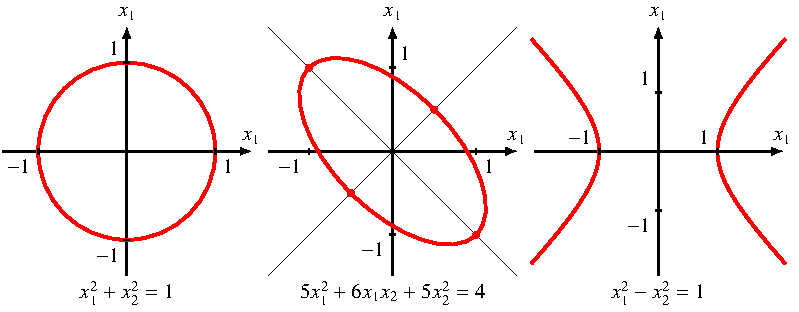
\includegraphics{chapters/010-skalarprodukt/images/kreise.pdf}
\caption{Kreise verschiedener Skalarprodukte in der Ebene.
Links der Kreis, der aus dem Standardskalarprodukt entsteht.
Rechts der zum hyperbolischen Skalarprodukt behörige ``Kreis'', er
besteht aus zwei Hyperbelästen.
Im Allgemeinen ist die Menge $\|v\|=1$ für die zu einem Skalarprodukt
gehörige Norm eine Ellipse, wie im mittleren Bild dargestellt.
\label{buch:skalarprodukt:definition:fig:kreise}}
\end{figure}
%

Verschiedene Skalarprodukte in zwei Dimensionen kann man durch ihre
zugehörten ``Kreise'' visualisieren
(Abbildung~\ref{buch:skalarprodukt:definition:fig:kreise}).
Damit meinen wir die Menge der Vektoren, die Norm $1$ haben.
Abbildung~\ref{buch:skalarprodukt:definition:fig:kreise} zeigt
die Kreise für drei verschiedene Skalarprodukte.
Links ist der Kreis für das Standard\-skalarprodukt $x_1y_1+x_2y_2$
dargestellt, der tatsächlich die Form eines Kreises hat.
Das Skalarprodukt von
Beispiel~\ref{buch:skalarprodukt:definition:bsp:hyperbolisch}
führt auf die Kurven mit der Gleichung
\[
x_1^2-x_2^2=1,
\]
dies sind Hyperbeln.
Es heisst daher auch das hyperbolische Skalarprodukt, obwohl es
\index{Skalarprodukt!hyperbolisch}
im strengen Sinne der
Definition~\ref{buch:skalarprodukt:definition:def:skalarprodukt}
kein Skalarprodukt ist.
In der Mitte schliesslich ist der Kreis für das Skalarprodukt 
\[
\langle x,y\rangle
=
2
\cdot
\frac{x_1+x_2}{\!\sqrt{2}}
\cdot
\frac{y_1+y_2}{\!\sqrt{2}}
+
\frac12
\cdot
\frac{x_1-x_2}{\!\sqrt{2}}
\cdot
\frac{y_1-y_2}{\!\sqrt{2}}
=
\frac{5x_1y_1 + 3x_1y_2 + 3x_2y_1 + 5x_2y_2}{2}
\]
dargestellt.
Die zugehörige Norm ist
\[
\|x\|^2
=
\frac14(
5x_1^2 + 5x_2^2 + 6x_1x_2).
\]
Der Kreis bestehen aus den Punkten einer Ellipse mit den Halbachsen
$1$ und $\frac12$, die um $45^\circ$ gegenüber den Koordinatenachsen
verdreht sind.
Diese Ellipse verläuft durch die Punkte $(\pm\frac12,\pm\frac12)$ und
$(\pm1,\mp1)$.

Für die Gram-Matrix $G$ eines Skalarproduktes bedeutet die Forderung,
dass das Skalarprodukt bilinear ist, dass die Matrix $G$ positiv
definit sein muss.
Aus der linearen Algebra ist bekannt, dass $G$ genau dann positiv
definit ist, wenn $G$ eine Cholesky-Zerlegung $G=L\transpose{L}$ hat,
deren Diagonalelemente alle positiv sind.

Ein Skalarprodukt hat jetzt alle Eigenschaften, die erlauben, einen 
Abstandsbegriff zu definieren.

\begin{definition}
\label{buch:skalarprodukt:definition:def:norm}
Die zu einem Skalarprodukt $\langle\;\,,\;\rangle$ gehörige Norm ist
definiert als
\[
\| v\|
=
\!\sqrt{\langle v,v\rangle}
\]
für $v\in V$.
\end{definition}

Die Norm erfüllt $\|\lambda v\| = |\lambda|\,\|v\|$ für jeden Vektor
$v\in V$ und $\lambda\in\mathbb{R}$.
In Worten bedeutet dies, dass bei der Skalierung eines Vektors die Norm
auf die gleiche Art skaliert.

%
% Sesquilineare Funktionen
%
\subsection{Sesquilineare Funktionen}
Sei jetzt $V$ ein komplexer Vektorraum.
Aus einer bilinearen Funktion
\[
b\colon V\times V \to \mathbb{C} : (u,v) \mapsto b(u,v)
\]
auf $V$ kann jedoch keine brauchbare Norm abgeleitet werden.
Eine solche müsste $\| v\|=b(v,v)\ge 0$ erfüllen.
Selbst wenn $b(u,u)> 0$ ist für einen speziellen Vektor $u\in V$,
ist das Skalarprodukt von $iu$ mit sich selbst
\[
b(iu,iu)
=
i^2 b(u,u)
=
-b(u,u)
<
0.
\]
Da $|i|=1$ ist, würde man eher erwarten, dass $iu$ die gleiche 
Länge hat wie $u$, dass also $b(iu,iu)=b(u,u)$.
Bilinearität funktioniert also nicht als Bedingung, um ein Skalarprodukt
zu konstruieren, für welches auch die geometrische Intuition des Abstands
anwendbar bleibt.

\begin{definition}
Eine Funktion $f\colon V\to U$ zwischen komplexen Vektorräumen 
heisst {\em konjugiert linear}, wenn 
\[
f(\lambda u + \mu v)
=
\overline{\lambda} f(u) + \overline{\mu} (v)
\]
ist für alle $u,v\in V$ und $\lambda,\mu\in \mathbb{C}$.
\end{definition}

Im obengenannten Beispiel wird $b(iu,iu)>0$, wenn $b$ im ersten Faktor
konjugiert linear ist.
Dann ist nämlich $b(iu,iu) = -ib(u,iu) = -i^2 b(u,u) = b(u,u)>0$.

\begin{definition}
Eine Funktion
\[
\langle\;\,,\;\rangle
\colon
V\times V \to \mathbb{C}
:
(u,v) \mapsto \langle u,v\rangle
\]
heisst {\em sesquilinear} oder {\em Sesquilinearform}
wenn sie linear ist im zweiten Argument
\end{definition}

Das lateinische Wort {\em sesqui} bedeudet eineinhalb, eine
sesquilineare Funktion ist linear in einem Faktor, aber nur
halb linear im anderen.

\begin{beispiel}
Die Form
\[
\langle u,v\rangle = \sum_{i=1}^n \overline{u}_i v_i
\]
mit $u,v\in \mathbb{C}^n$ ist sesquilinear.
Tatsächlich gilt
\begin{align*}
\langle u,\lambda v+\mu w\rangle
&=
\sum_{i=1}^n \overline{u}_i (\lambda v_i+\mu w_i)
=
\lambda
\sum_{i=1}^n \overline{u}_i v_i
+
\mu
\sum_{i=1}^n \overline{u}_i w_i
=
\lambda\langle u,v\rangle
+
\mu\langle u,w\rangle
\\
\langle \lambda u+\mu w, v\rangle
&=
\sum_{i=1}^n \overline{(\lambda u_i+\mu w_i)}v_i
=
\overline{\lambda}
\sum_{i=1}^n \overline{u}_i v_i
+
\overline{\mu}
\sum_{i=1}^n \overline{w}_iv_i
=
\overline{\lambda}\langle u,v\rangle
+
\overline{\mu}\langle w,v\rangle.
\qedhere
\end{align*}
\end{beispiel}

Eine Sesquilinearform auf einem endlichdimensionalen Vektorraum $V$
kann wie im reellen Fall mit Hilfe einer Matrix beschrieben werden.
Eine Darstellung der Vektoren $u$ und $v$ mit Koordinaten $u_i$ und
$v_i$ in der Basis $b_1,\dots,b_n\in V$ führt auf das Skalarprodukt
\[
f(u,v)
=
f\biggl( \sum_{i=1}^n u_ib_i, \sum_{k=1}^n v_kb_k \biggr)
=
\sum_{i=1}^n\sum_{k=1}^n
\overline{u}_i
\underbrace{f(b_i, b_k)}_{\displaystyle=h_{ik}}
v_k.
\]
In Matrixform mit der Matrix $H$ mit Einträgen $h_{ik}$ ist dies
gleichbedeutend mit
\[
f(u,v)
=
\transpose{
\begin{pmatrix}
\overline{u}_1\\
\overline{u}_2\\
\vdots\\
\overline{u}_n
\end{pmatrix}
}
H
\begin{pmatrix}
v_1\\v_2\\\vdots\\v_n
\end{pmatrix}.
\]
Der transponierte Vektor $\transpose{\overline{u}}$ mit komplex
konjugierten Einträgen heisst auch konjugiert transponiert zu $u$.

\begin{definition}
Ist $A\in M_{m\times n}(\mathbb{C})$ eine komplexe $m\times n$-Matrix.
Die Matrix $\overline{A}\in M_{m\times n}(\mathbb{C})$ mit 
den komplex konjugierten Matrixelementen von $A$ heisst die
(komplex) konjugierte Matrix zu $A$.
\index{komplex konjugierte Matrix}%
\index{konjugierte Matrix}%
Die Matrix 
\[
A^*
=
\transpose{\overline{A}}
=
\transpose{
\begin{pmatrix}
\overline{a_{11}}&\overline{a_{12}}&\dots &\overline{a_{1n}}\\
\overline{a_{21}}&\overline{a_{22}}&\dots &\overline{a_{2n}}\\
\vdots           &\vdots           &\ddots&\vdots           \\
\overline{a_{m1}}&\overline{a_{m2}}&\dots &\overline{a_{mn}}
\end{pmatrix}
}
=
\begin{pmatrix}
\overline{a_{11}}&\overline{a_{21}}&\dots &\overline{a_{n1}}\\
\overline{a_{12}}&\overline{a_{22}}&\dots &\overline{a_{n2}}\\
\vdots           &\vdots           &\ddots&\vdots           \\
\overline{a_{1m}}&\overline{a_{2m}}&\dots &\overline{a_{nm}}
\end{pmatrix}
\in
M_{n\times m}(\mathbb{C})
\]
heisst die {\em transponiert konjugierte} oder {\em hermitesch konjugierte}
\index{hermitesch konjugiert}%
Matrix.
\end{definition}

Eine Sesquilinearform kann immer geschrieben werden als
\(
f(u,v) = u^*Hv
\)
mit einer hermiteschen Matrix $H$.

%
% Hermitesche Formen
%
\subsection{Hermitesche Formen}
Damit aus einer sesquilinearen Funktion eine Norm abgeleitet werden
kann, muss das Produkt $\langle u,u\rangle$ für jeden Vektor $u\in V$
eine reelle Zahl sein.
Selbst für die sesquilineare Funktion
\[
\langle\;\,,\;\rangle
\colon
\mathbb{C}\times\mathbb{C}
\to
\mathbb{C}
:
(u,v) \mapsto i\overline{u}v
\]
ist dies jedoch nicht der Fall, da $\langle 1,1\rangle = i\not\in\mathbb{R}$
ist.
Die folgende Eigenschaft kann aber garantieren, dass
$\langle u,u\rangle\in\mathbb{R}$.

\begin{definition}
Eine sesquilinear Funktion 
\[
\langle \;\,,\;\rangle
\colon
V\times V
\to
\mathbb{C}
\]
heisst in {\em konjugiert symmetrisch} oder {\em hermitesch}, wenn
\index{konjugiert symmetrisch}%
\index{hermitesch!Sesquilinearform}%
\[
\langle u,v\rangle = \overline{\langle v,u\rangle}
\]
für alle $u,v\in V$ gilt.
\end{definition}

\begin{beispiel}
Die Standard-Sesquilinearform
\[
\langle u,v\rangle
=
\sum_{i=1}^n \overline{u}_i v_i
\]
auf $V=\mathbb{C}^n$ ist konjugiert symmetrisch, denn
\begin{align*}
\langle u,v\rangle
&=
\sum_{i=1}^n \overline{u}_i v_i
=
\overline{
\sum_{i=1}^n u_i \overline{v}_i
}
=
\overline{\langle v,u\rangle}.
\qedhere
\end{align*}
\end{beispiel}

Die Gram-Matrix einer hermitesche Sesquilinearform hat die Matrix-Elemente
\[
h_{ik}
=
\langle b_i,b_k\rangle
=
\overline{\langle b_k,b_i\rangle}
=
\overline{h}_{ki}
\qquad\Rightarrow\qquad
H^* = H.
\]
Man sagt auch, die Matrix $H$ ist {\em hermitesch}.
\index{hermitesch!Matrix}%

%
% Komplexe Skalarprodukte
%
\subsection{Komplexe Skalarprodukte}
Wie bei einem reellen Skalarprodukt reichen auch im Fall eines
komplexen Vektorraums die Eigenschaften der Sesquilinearität
und der hermiteschen Symmetrie nicht aus, ein sinnvolles
Skalarprodukt zu definieren.

\begin{definition}
Eine hermitesche Sesquilinearform $\langle\;\,,\;\rangle$
auf dem komplexen Vektorraum $V$ heisst {\em positiv definit}, wenn
\[
\langle u,u\rangle > 0
\]
gilt für alle $u\ne 0$ in $V$.
Ein {\em komplexes Skalarprodukt} ist eine positiv definite hermitesche
Sesquilinearform.
Die zugehörige {\em Norm} eines Vektors ist
$\|v\| = \!\sqrt{\langle u, u\rangle}$.
\end{definition}

Auch für ein komplexes Skalarprodukt gilt die Skalierungseigenschaft
\[
\|\lambda v\|^2
=
\langle \lambda v,\lambda v\rangle
=
\overline{\lambda}\lambda\langle v,v\rangle
=
|\lambda|^2\,\|v\|^2
\qquad\Rightarrow\qquad
\|\lambda v\|
=
|\lambda|\, \|v\|,
\]
ganz analog zur entsprechenden Skalierungseigenschaft für ein
reelles Skalarprodukt.





